%%%%%%%%%%%%%%%%%%%%%%%%%%%%%%%%%%%%%%%%%
% Structured General Purpose Assignment
% LaTeX Template
%
% This template has been downloaded from:
% http://www.latextemplates.com
%
% Original author:
%  Ted Pavlic (http://www.tedpavlic.com)
% Modified by:
%  Joe Del Rocco (https://joe.delrocco.org)
%%%%%%%%%%%%%%%%%%%%%%%%%%%%%%%%%%%%%%%%%

%----------------------------------------------------------------------------------------
%  PACKAGES AND CONFIGURATION
%----------------------------------------------------------------------------------------

\documentclass[fleqn]{article}
\usepackage{geometry}
\usepackage{fancyhdr} % For custom headers
\usepackage{lastpage} % To determine the last page for the footer
\usepackage{extramarks} % For headers and footers
\usepackage[most]{tcolorbox} % For problem answer sections
\usepackage[utf8]{inputenc}
\usepackage{graphicx} % For inserting images
\usepackage{xcolor} % For link coloring
\usepackage[hidelinks]{hyperref} % For URL links (no box or color name)

% Margins
\geometry{
a4paper,
tmargin=1in,
bmargin=1in,
lmargin=1in,
rmargin=1in,
textwidth=6.5in,
textheight=9.0in,
headsep=0.25in
}

% Header and footer
\pagestyle{fancy}
\lhead{} % Top left header
\lhead{\myCourse: \myAssignment} % Top center header
\rhead{\firstxmark} % Top right header
\lfoot{\lastxmark} % Bottom left footer
\cfoot{} % Bottom center footer
\rfoot{Page\ \thepage\ of\ \pageref{LastPage}} % Bottom right footer
\renewcommand\headrulewidth{0.4pt} % Size of the header rule
\renewcommand\footrulewidth{0.4pt} % Size of the footer rule

% Other configurations
\setlength\parindent{0pt} % Removes all indentation from paragraphs
\setlength\parskip{1pt} % Ensures paragraphs are still recognizable as such
\setcounter{secnumdepth}{0} % Removes default section numbers
\setcounter{tocdepth}{3} % Sets depth of table of contents
\linespread{1.1}

% Template values
\newcommand{\myLogo}{hu-logo.jpg}
\newcommand{\myName}{Abeer Khan}
\newcommand{\myJobTitle}{ak05419}
\newcommand{\myCompany}{Habib University}
\newcommand{\myCourse}{CS 451 - Computational Intelligence}
\newcommand{\mySection}{Spring 2022}
\newcommand{\myAssignment}{Travelling Salesman Problem using EA}
\newcommand{\myDueDate}{Sunday,\ February\ 13,\ 2022}

%----------------------------------------------------------------------------------------
%  DOCUMENT STRUCTURE (MACROS & ENVIRONMENTS)
%----------------------------------------------------------------------------------------

% Colored links macro
\newcommand{\hrefcol}[3] {\href{#1}{\textcolor{#3}{#2}}}

% Creates a counter to keep track of the number of problems
\newcounter{homeworkProblemCounter}

% Macro for custom title page signature header
\newsavebox{\myTitleSignature}
\sbox{\myTitleSignature}{%
\begin{tabular*}{\textwidth}{@{}l@{}|@{\extracolsep{0.125in}}l@{}}%
\parbox{4.25in}{\raggedright{\includegraphics{\myLogo}}} &
\parbox[c][]{2.5in}{{\textbf{\myName} \par}
                    {\small \myJobTitle \par}
                    {\small \myCompany \par}
                    {\small \myLocation \par}
                    {\small \hrefcol{https://\myURL}{\myURL}{blue} \par}
                    {\small \hrefcol{mailto:\myEmail}{\myEmail}{blue}} \par}
\end{tabular*}}

% Header and footer for when a page split occurs within a problem environment
\newcommand{\enterProblemHeader}[1]{%
\nobreak\extramarks{#1}{#1 continued on next page\ldots}\nobreak%
}

% Header and footer for when a page split occurs between problem environments
\newcommand{\exitProblemHeader}[1]{%
\nobreak\extramarks{#1 (continued)}{#1 continued on next page\ldots}\nobreak%
\nobreak\extramarks{#1}{}\nobreak%
}

\newcommand{\homeworkProblemName}{} % Argument = name of problem; default = "Problem #"
\newenvironment{homeworkProblem}[1][Problem \arabic{homeworkProblemCounter}]{%
\stepcounter{homeworkProblemCounter}% % Increase counter for number of problems
\renewcommand{\homeworkProblemName}{#1}% % Assign \homeworkProblemName the argument
\section{\homeworkProblemName}% % Make a section in the document with the custom problem count
\enterProblemHeader{\homeworkProblemName}% % Header and footer within environment
}{%
\exitProblemHeader{\homeworkProblemName}% % Header and footer after environment
}

\newcommand{\problemAnswer}[1]{ % Defines the problem answer command with the content as the only argument
\begin{tcolorbox}[breakable,enhanced,colback=gray!5!white,title=Answer]%
#1
\end{tcolorbox}%
% Alternative - Makes the box around the problem answer and puts the content inside
%\noindent\framebox[\columnwidth][c]{\begin{minipage}{0.98\columnwidth}#1\end{minipage}}
}

\newcommand{\homeworkSectionName}{}
\newenvironment{homeworkSection}[1]{% % For sections w/in problems; Argument = name of section (no default)
\renewcommand{\homeworkSectionName}{#1}% % Assign \homeworkSectionName the argument
\subsection{\homeworkSectionName}% % Make a subsection with the name of the subsection
% \enterProblemHeader{\homeworkProblemName\ [\homeworkSectionName]}% % Header and footer within environment
% }{%
\enterProblemHeader{\homeworkProblemName}% % Header and footer after environment
}

%----------------------------------------------------------------------------------------
%   TITLE PAGE
%----------------------------------------------------------------------------------------
\begin{document}

% Blank out the traditional title page
\title{\vspace{-1in}} % no title name
\author{} % no author name
\date{} % no date listed
\maketitle % makes this a title page

% Use custom title macro instead
\usebox{\myTitleSignature}
\vspace{1in} % spacing below title header

% Assignment title
{\centering \huge \myAssignment \par}
{\centering \noindent\rule{4in}{0.1pt} \par}
\vspace{0.05in}
{\centering \myCourse~: \mySection~ \par}
{\centering \myDueDate \par}
%{\centering Prepared w/ \LaTeX \par}
\vspace{1in}

% Table of Contents
\newpage
\tableofcontents
\newpage

%----------------------------------------------------------------------------------------
%	PROBLEM 1
%----------------------------------------------------------------------------------------

%\begin{homeworkProblem}[Exercise \#\arabic{homeworkProblemCounter}] % Use for custom section title
\begin{homeworkProblem}{}


%-----------------------------------------------

%\begin{homeworkSection}{\homeworkProblemName:~(a)} % Use for repeating problem name
\begin{homeworkSection}{Travelling Salesman: Problem Formulation}
The travelling salesman problem is a well-known optimization problem that when given a list of cities/destinations, involves finding the shortest and most efficient route that visits each destination exactly once. An optimal solution could be located using meta-heuristic optimization techniques.  \par

For this problem, the Qatar dataset was used for finding the optimal solution using an Evolutionary Algorithm. The dataset is comprised of 194 cities/nodes - with each city having it's set of x, and y co-ordinates. Using this, an adjacency list is created to construct the many permutations of possible routes that visit each destination in this instance exactly once. The algorithm generates a random population of possible routes initially, which is then used for parent selection to generate offsprings, based on some parent selection scheme. After a mutation operator is applied onto an offspring, a fitness function is used to calculate the total distances of every chromosome in the population. Based on some survivor selection scheme, the fitness values are evaluated to choose the individuals that will become a part of the population that will be carried onto the next generation. This is continued for a period of time, based on the parameters specified, and the best smallest distance found so far would be the output. The algorithm is implemented using a Python class.
\end{homeworkSection}

%-----------------------------------------------

\begin{homeworkSection}{Chromosome Representation}
In our population, a chromosome for this problem would represent the many permutations of possible routes that visit each destination exactly once. Each destination in our data-set has its set of x and y-co-ordinates. To calculate the distance between two destinations, we apply the Euclidean distance formula. \par
\end{homeworkSection}

%-----------------------------------------------

\begin{homeworkSection}{Fitness Function}
The fitness function determines the total distance between each destination in each chromosome in the population. The fitness value of the chromosome will be considered high, if the total distance of the chromosome is small. As the value of the total distance grows smaller, the fitness value of the chromosome increases. \par
\end{homeworkSection}

%-----------------------------------------------

\begin{homeworkSection}{Parameters Used}
The following parameters are implemented in our program with some constant values that ensure fair comparison between all iterations of our algorithm. They can be changed to observe the behavior of our algorithm:\\
\begin{itemize}
    \item Population size: $300$
    \item Number of offspring to be produced in each generation: $500$
    \item No. of generations: $50$
    \item Mutation rate: $0.7$
    \item No of Iterations: $10$
\end{itemize}\par
\end{homeworkSection}

%-----------------------------------------------
\newpage
\begin{homeworkSection}{Results: Single Combination}
We repeated the EA process for the following single combinations of parent and survivor selections respectively:\\
\begin{itemize}
    \item FPS and FPS:\\
    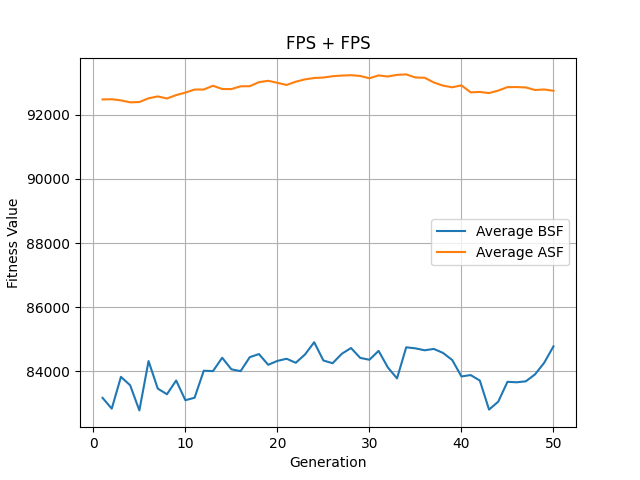
\includegraphics[scale=0.7]{Images/tsp_fps_fps.png}
    
    \item Truncation and Truncation:\\
    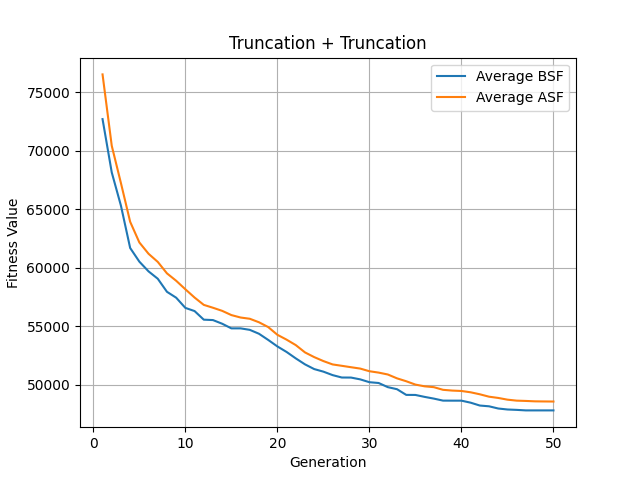
\includegraphics[scale=0.7]{Images/tsp_t_t.png}
    \newpage
    
    \item Random and Random:\\
    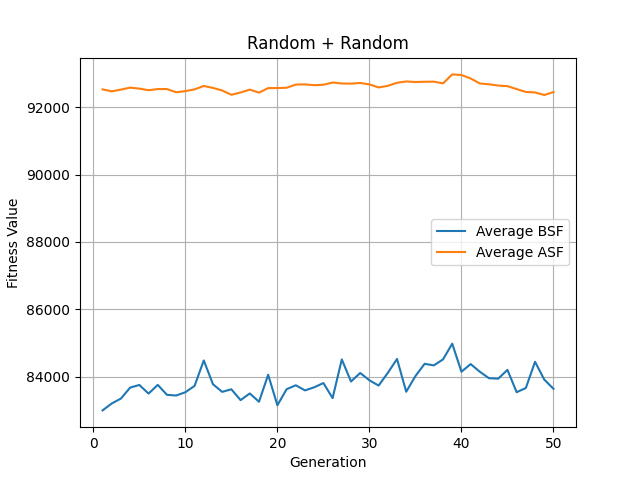
\includegraphics[scale=0.7]{Images/tsp_r_r.png}
    
    
    \item RBS and RBS:\\
    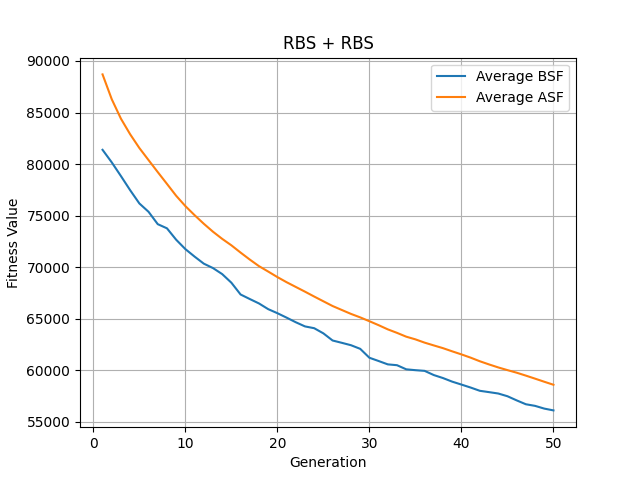
\includegraphics[scale=0.7]{Images/tsp_rbs_rbs.png}
    
\end{itemize}\par
\end{homeworkSection}

%-----------------------------------------------
\newpage
\begin{homeworkSection}{Results: Different Combinations (FPS)}
We repeated the EA process for the following combinations of parent and survivor selections respectively:\\
\begin{itemize}
    \item FPS and Truncation:\\
    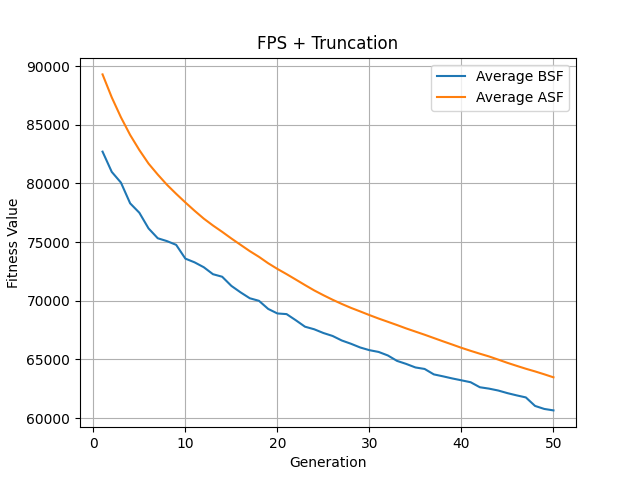
\includegraphics[scale=0.7]{Images/tsp_fps_t.png}
    
    \item FPS and Random:\\
    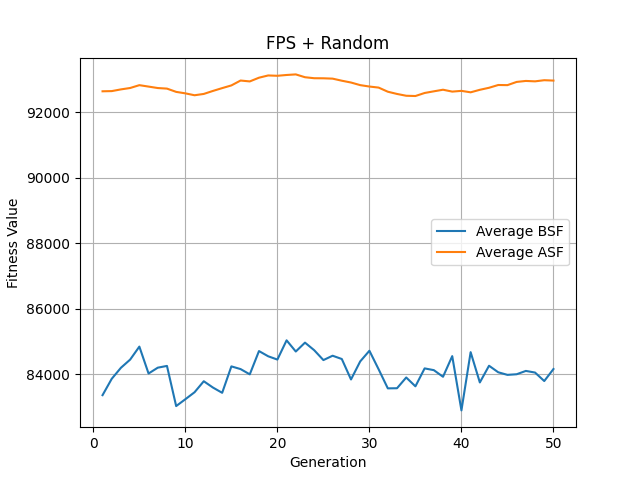
\includegraphics[scale=0.7]{Images/tsp_fps_r.png}
    
    \newpage
    
    \item FPS and RBS:\\
    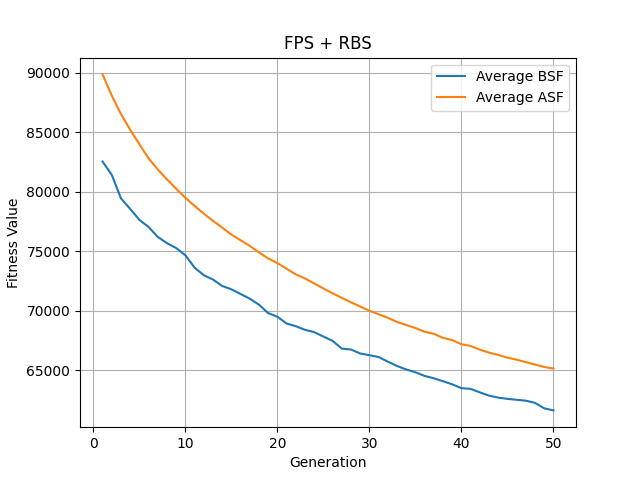
\includegraphics[scale=0.7]{Images/tsp_fps_rbs.png}

\end{itemize}\par
\end{homeworkSection}

%-----------------------------------------------
\newpage
\begin{homeworkSection}{Results: Different Combinations (Random)}
We repeated the EA process for the following combinations of parent and survivor selections respectively:\\
\begin{itemize}
    \item Random and Truncation:\\
    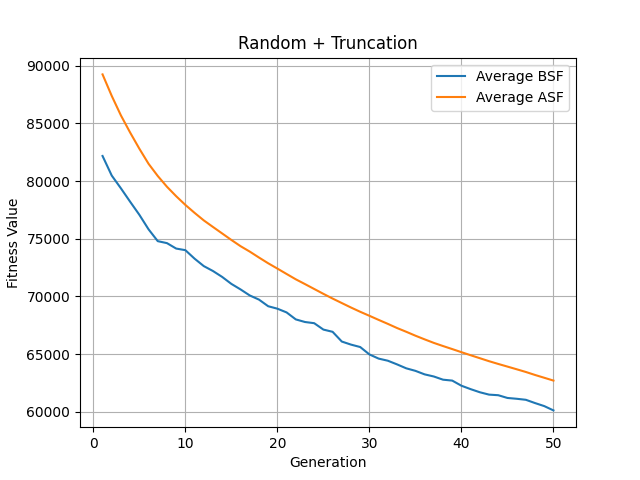
\includegraphics[scale=0.7]{Images/tsp_r_t.png}
    
    \item Random and FPS:\\
    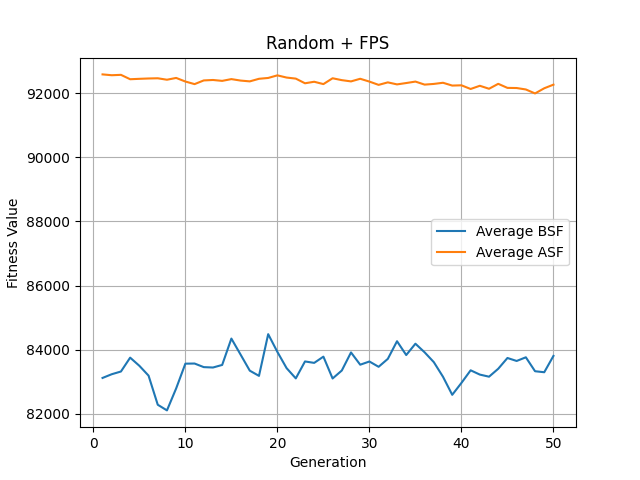
\includegraphics[scale=0.7]{Images/tsp_r_fps.png}
    
    \newpage
    
    \item Random and RBS:\\
    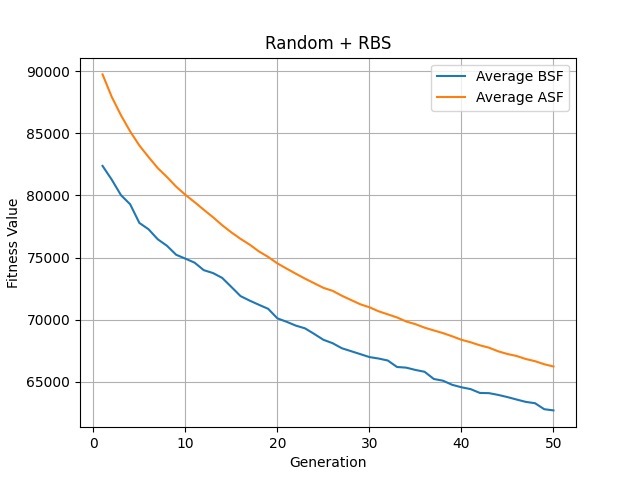
\includegraphics[scale=0.7]{Images/tsp_r_rbs.png}

\end{itemize}\par
\end{homeworkSection}

%-----------------------------------------------
\newpage
\begin{homeworkSection}{Results: Different Combinations (Truncation)}
We repeated the EA process for the following combinations of parent and survivor selections respectively:\\
\begin{itemize}
    \item Truncation and Random:\\
    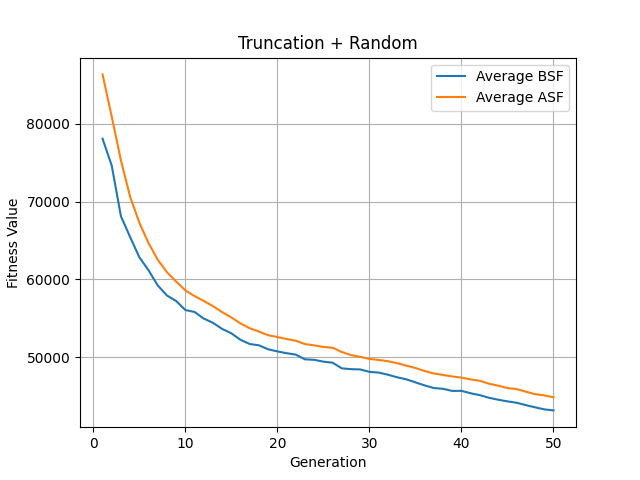
\includegraphics[scale=0.7]{Images/tsp_t_r.png}
    
    \item Truncation and FPS:\\
    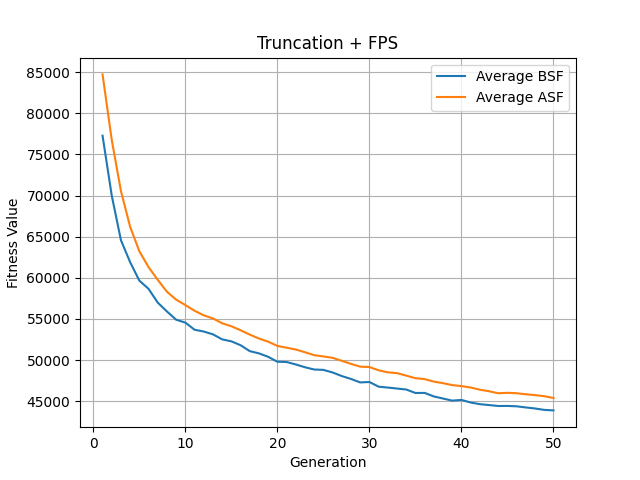
\includegraphics[scale=0.7]{Images/tsp_t_fps.png}
    
    \newpage
    
    \item Truncation and RBS:\\
    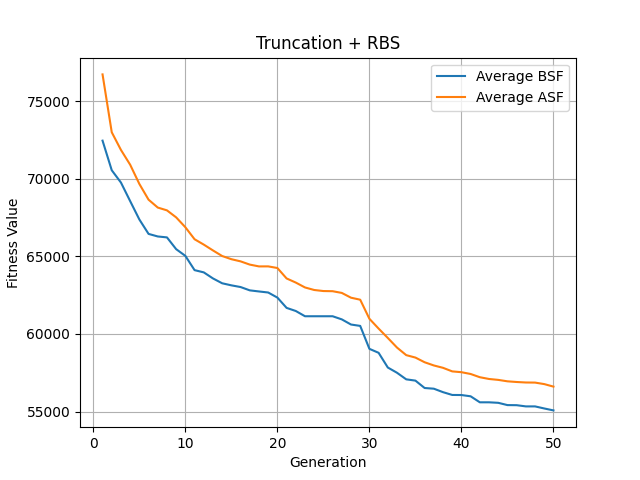
\includegraphics[scale=0.7]{Images/tsp_t_rbs.png}

\end{itemize}\par
\end{homeworkSection}

%-----------------------------------------------
\newpage
\begin{homeworkSection}{Results: Different Combinations (RBS)}
We repeated the EA process for the following combinations of parent and survivor selections respectively:\\
\begin{itemize}
    \item RBS and Truncation:\\
    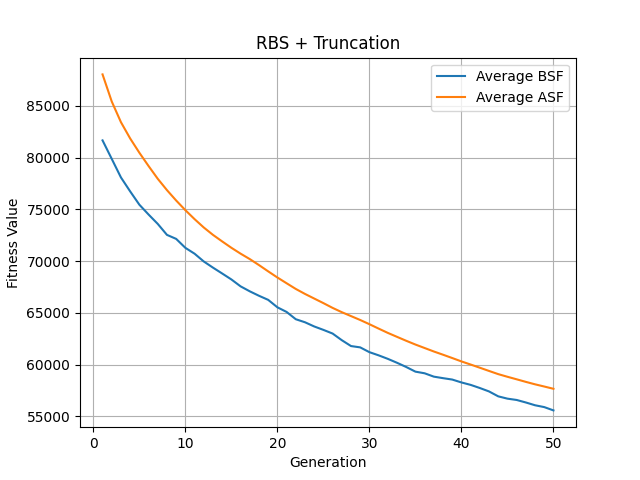
\includegraphics[scale=0.7]{Images/tsp_rbs_t.png}
    
    \item RBS and FPS:\\
    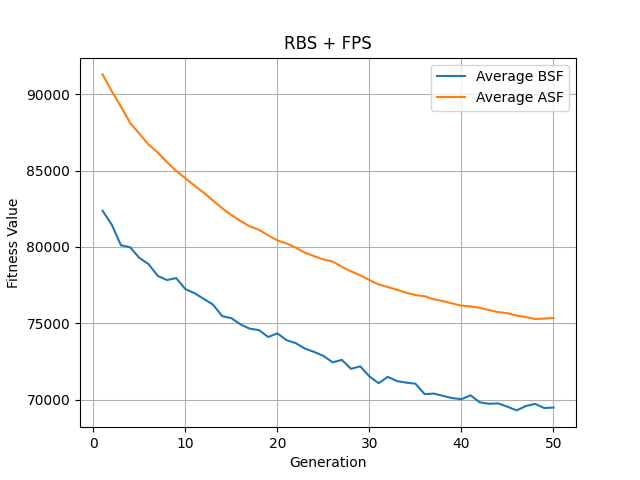
\includegraphics[scale=0.7]{Images/tsp_rbs_fps.png}
    
    \newpage
    
    \item RBS and Random:\\
    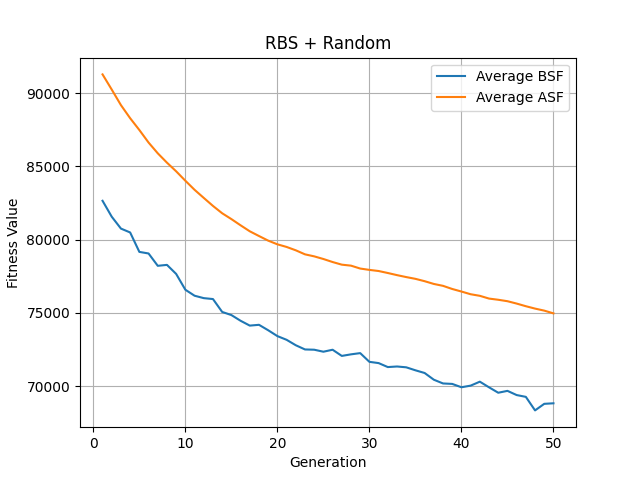
\includegraphics[scale=0.7]{Images/tsp_rbs_r.png}

\end{itemize}\par
\end{homeworkSection}

%-----------------------------------------------
\newpage
\begin{homeworkSection}{Analysis and Findings}
Analysis of the graphs leads to the following conclusions:\par
\newline
a) The Truncation and FPS parent and survivor selection scheme combination yields the best results when compared to other combinations of selection schemes. It converges to a total distance of around forty-five thousand. Furthermore, there is a very small difference between the averages of the average fitness values and average best fitness values. According to this, we can conclude that Truncation and FPS would be the best parent and survivor selection scheme combination for this problem. 
\newline

b) Certain parent and survivor selection scheme combinations such as FPS and FPS, Random and Random, FPS and Random, and Random and FPS, do not yield very good results. Furthermore, there is a very large difference between the averages of the average fitness values and average best fitness values. They converge to very high values of total distance, which is not a good solution for this problem as we need to find the shortest overall distance. 
\newline

After concluding that the Truncation and FPS parent and survivor selection scheme combination can yield the best results, the generation parameter was changed from 50 to 200 to observe how small the best fitness value can become over a period of time. The best fitness value generated was calculated to be at 35693. 

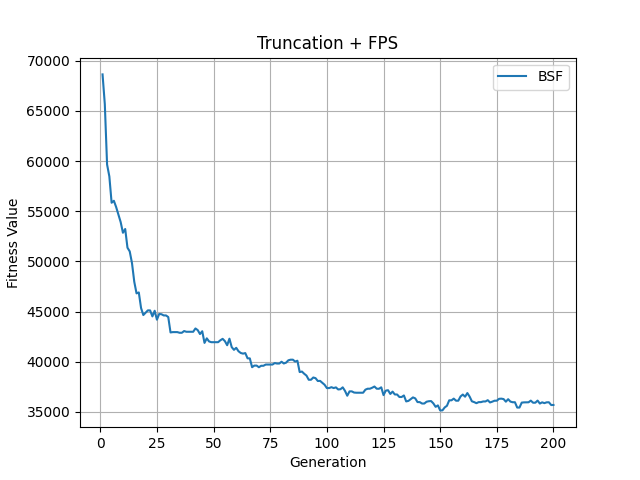
\includegraphics[scale=0.7]{Images/tsp_best_t.png}

\end{homeworkSection}
\end{homeworkProblem}
\end{document}
%----------------------------------------------------------------------------------------
%	DONE
%----------------------------------------------------------------------------------------
